% This file was created by matlab2tikz v0.4.7 running on MATLAB 7.14.
% Copyright (c) 2008--2014, Nico Schlömer <nico.schloemer@gmail.com>
% All rights reserved.
% Minimal pgfplots version: 1.3
% 
% The latest updates can be retrieved from
%   http://www.mathworks.com/matlabcentral/fileexchange/22022-matlab2tikz
% where you can also make suggestions and rate matlab2tikz.
% 

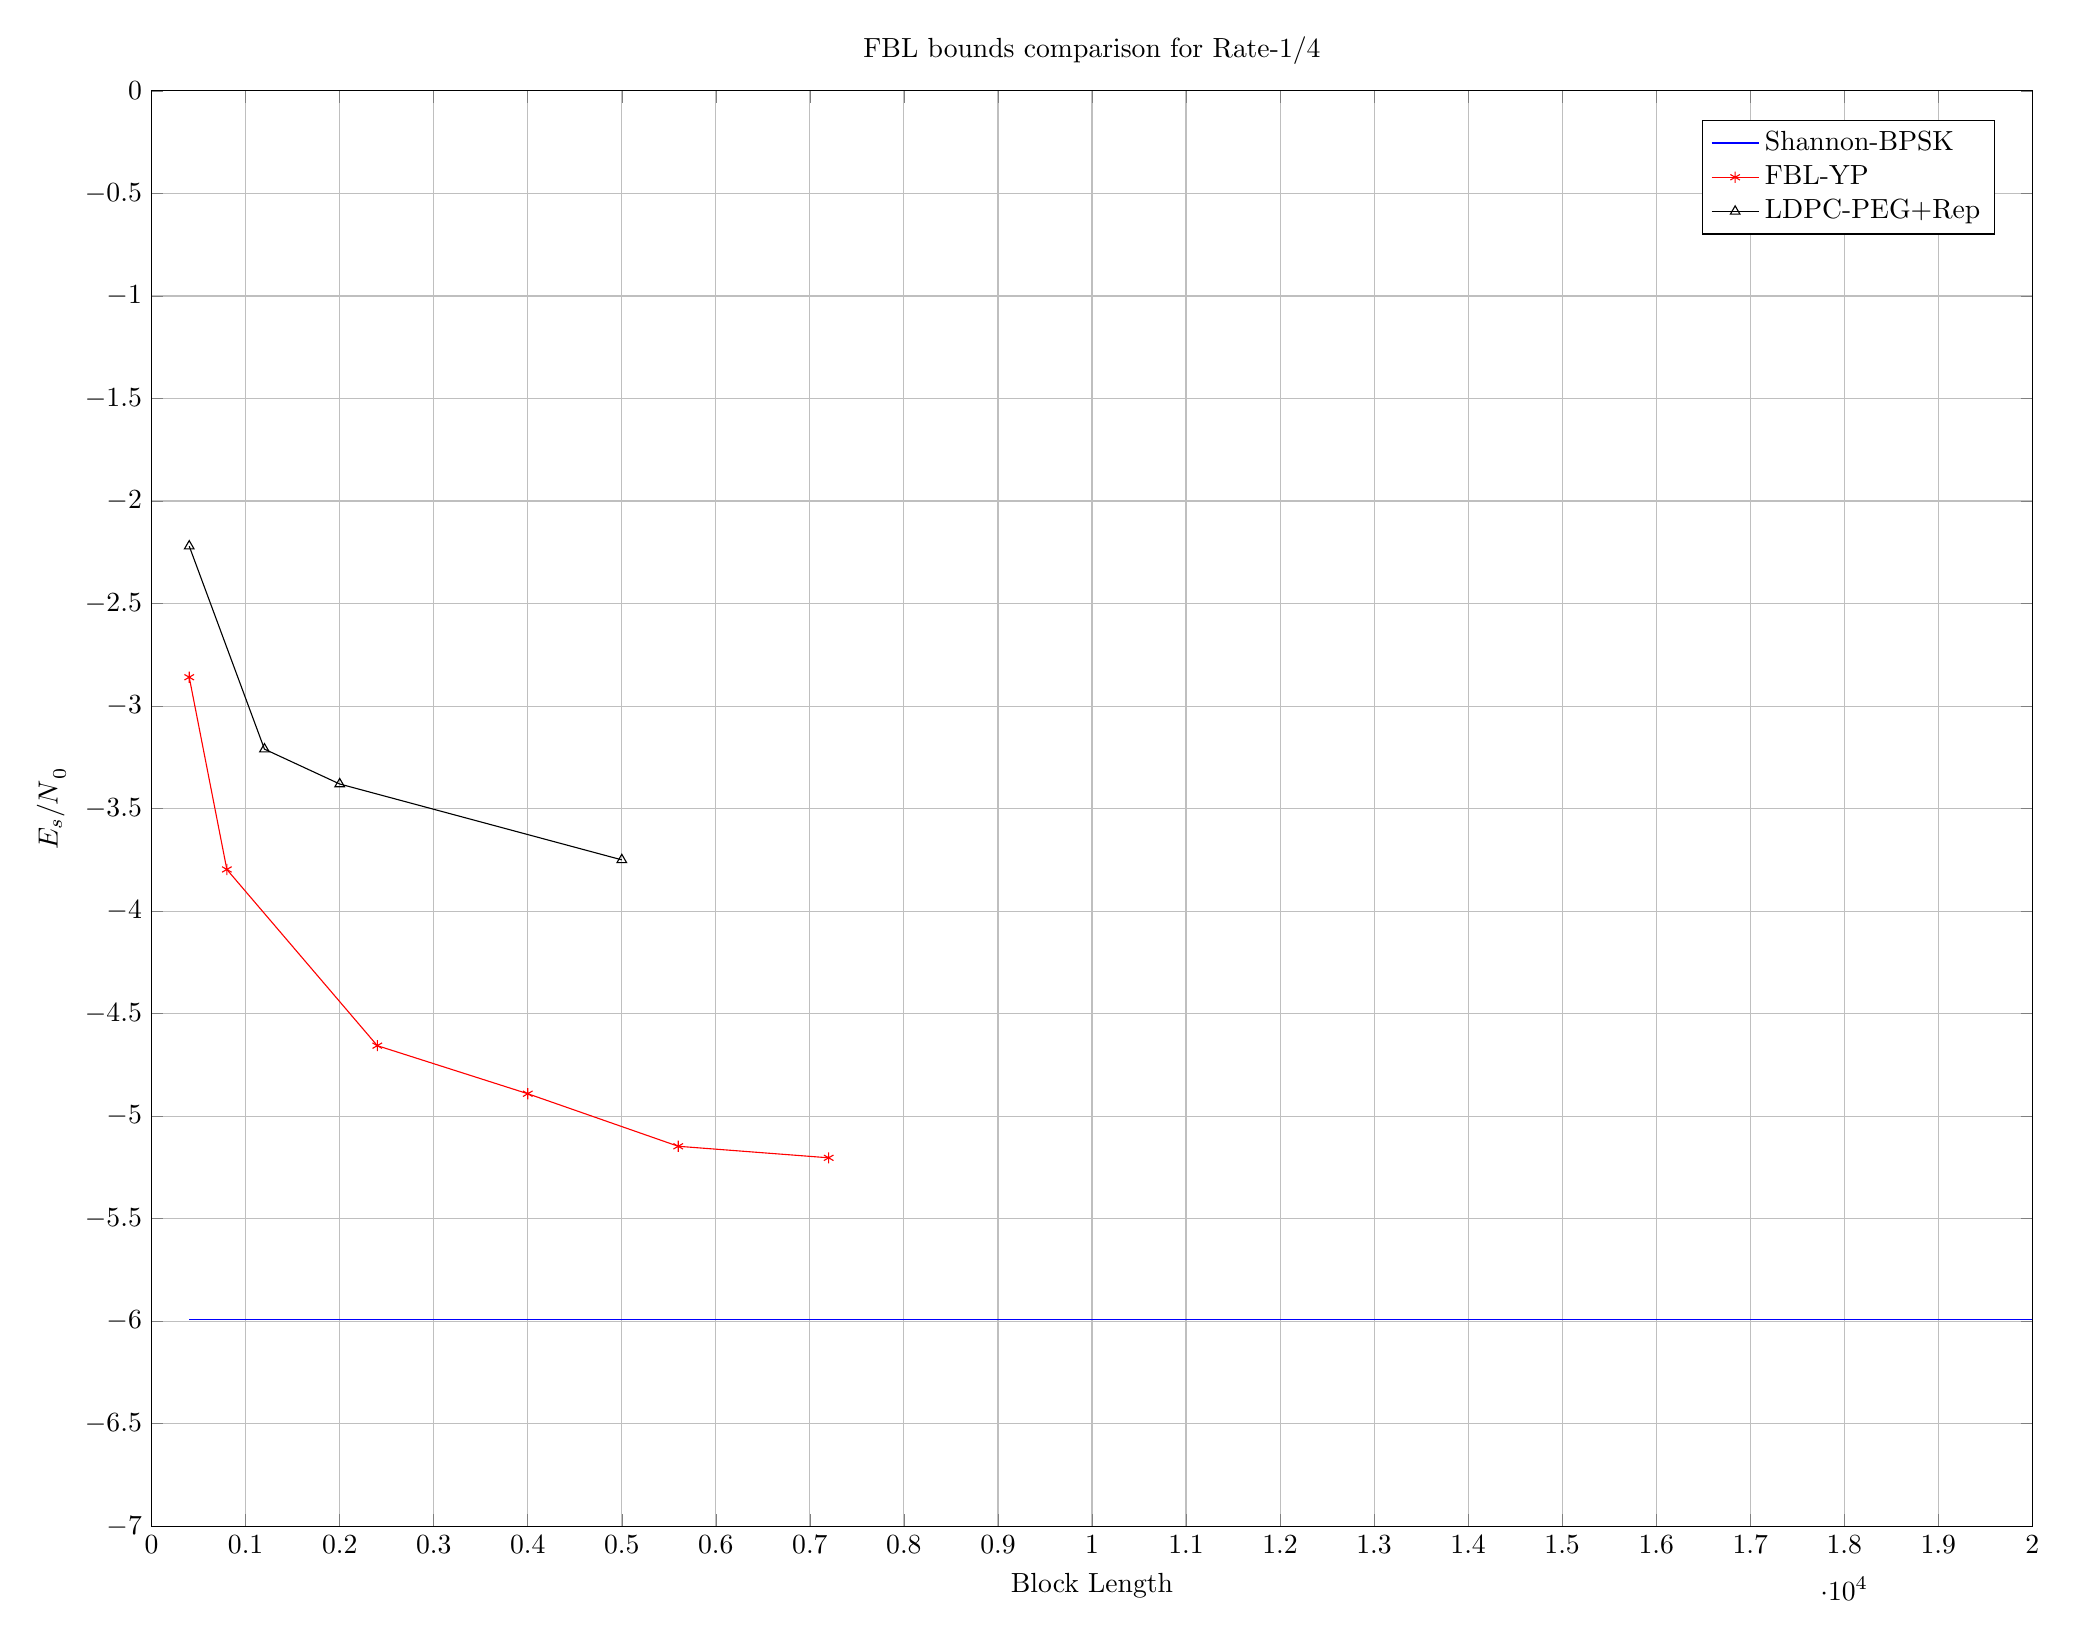
\begin{tikzpicture}
\begin{axis}[%
width=9.40357064741907in,
height=7.17652777777778in,
scale only axis,
xmin=0,
xmax=20000,
xlabel={Block Length},
xmajorgrids,
ymin=-7,
ymax=0,
ylabel={$\text{E}_\text{s}\text{/N}_\text{0}$},
ymajorgrids,
title={FBL bounds comparison for Rate-1/4},
legend style={draw=black,fill=white,legend cell align=left}
]

\addplot [color=blue,solid]
  table[row sep=crcr]{
400	  -5.99\\
500	  -5.99\\
1000  -5.99\\
5000	-5.99\\
10000	-5.99\\
15000	-5.99\\
20000	-5.99\\
};
\addlegendentry{Shannon-BPSK};

\addplot [color=red,solid,mark=asterisk,mark options={solid}]
  table[row sep=crcr]{400	-2.8594\\
800	-3.7969\\
2400	-4.6562\\
4000	-4.8906\\
5600	-5.1469\\
7200	-5.2031\\
};
\addlegendentry{FBL-YP};

\addplot [color=black,solid,mark=triangle,mark options={solid}]
  table[row sep=crcr]{400	-2.22\\
1200	-3.21\\
2000	-3.38\\
5000	-3.75\\
};
\addlegendentry{LDPC-PEG+Rep};

\end{axis}
\end{tikzpicture}
